\documentclass{article}

\usepackage{arxiv}

\usepackage[utf8]{inputenc} % allow utf-8 input
\usepackage[T1]{fontenc}    % use 8-bit T1 fonts
\usepackage{hyperref}       % hyperlinks
\usepackage{url}            % simple URL typesetting
\usepackage{booktabs}       % professional-quality tables
\usepackage{amsfonts}       % blackboard math symbols
\usepackage{nicefrac}       % compact symbols for 1/2, etc.
\usepackage{microtype}      % microtypography
\usepackage{lipsum}
\usepackage{graphicx}
\usepackage{import}
\graphicspath{ {./images/} }


\title{TP 1.2 - ESTUDIO ECONÓMICO-MATEMÁTICO DE APUESTAS EN LA RULETA}


\author{
    Abud Santiago Elias \\
    Legajo 47015 \\
    \texttt{ sabudvicco@gmail.com} \\
    %% examples of more authors
    \And
    Buchhamer Ariel \\
    Legajo 46217\\
    \texttt{arielbuchhamer1@outlook.com} \\
    \And
    Castellano Marcelo \\
    Legajo 39028 \\
    \texttt{marce.geek22@gmail.com} \\
    \And
    Dolan Guillermo Patricio \\
    Legajo 46101\\
    \texttt{guillermo230899@gmail.com} \\
    \And
    Navarro Franco \\
    Legajo 46387 \\
    \texttt{franconavarro1889@gmail.com} \\
%% \AND
%% Coauthor \\
%% Affiliation \\
%% Address \\
%% \texttt{email} \\
%% \And
%% Coauthor \\
%% Affiliation \\
%% Address \\
%% \texttt{email} \\
%% \And
%% Coauthor \\
%% Affiliation \\
%% Address \\
%% \texttt{email} \\
}

\usepackage[spanish]{babel}
\begin{document}
    \maketitle
    \begin{abstract}
        El siguiente documento tiene por objetivo analizar diferentes estrategias de apuestas.
        Las estrategias elegidas son:
        \begin{itemize}
          \item Martingala %Método de apuesta muy popular desde el siglo XVIII, la edad dorada de la ruleta francesa. Básicamente se trata de que cada vez que apuestes y pierdas vuelvas a apostar por el total de lo perdido desde que empezaste la sesión de juego.
          \item D'Alembert %ue perfilado en el siglo XVIII por Jean Baptiste le Rond D’Alembert, célebre matemático francés a quien debe su nombre
          \item Fibonacci
        \end{itemize}
        Se las evaluará teniendo en cuenta dos supuestos distintos:
        \begin{itemize}
          \item Capital infinito: Los jugadores jugarán hasta que terminen una cantidad especificada de jugadas.
          \item Capital acotado: Los jugadores poseen una cantidad definida de dinero al comenzar a apostar.
          La simulación podrá terminar tanto tras una cantidad de jugadas como cuando el jugador se quede sin dinero.
        \end{itemize}
    \end{abstract}

    \keywords{
    Simulación \and Ruleta \and Apuestas \and Estrategias
    }



% keywords can be removed
%\keywords{First keyword \and Second keyword \and More}


    \section{Introducción}
    La ruleta es un juego de azar típico de los casinos, cuyo nombre viene del término francés roulette,
    que significa ``ruedita'' o ``rueda pequeña''. Su uso como elemento de juego de azar, aún
    en configuraciones distintas de la actual, no está documentado hasta bien entrada la Edad Media.
    Es de suponer que su referencia más antigua es la llamada Rueda de la Fortuna, de la que hay
    noticias a lo largo de toda la historia, prácticamente en todos los campos del saber humano.

    Una ruleta posee un sistema de apuestas denominado "Martingala", que es un sistema de apuestas progresivo,
    en el cual se dobla la apuesta tras una pérdida, y se continúa jugando normalmente si se gana.

    Por otro lado, también se tiene el sistema D'Alembert, que es mucho más seguro que el método anterior.
    Este sistema se usa principalmente cuando se apuesta a las apuestas exteriores,
    es decir rojo/negro, par/impar, y 1-18/19-36. La asunción básica de esta estrategia de apuestas en ruleta,
    es que los aciertos en las apuestas exteriores en el largo plazo acabarán balanceándose.
    Así que si hay por ejemplo, una racha de rojos, es algo que solo puede ser temporal.
    Al final, el rojo y el negro acabarán más o menos a la par.

    Otro de los métodos que posee la ruleta, es el sistema Fibonacci, el cual es una de las estrategias
    más famosas y más exitosas entre los jugadores. Este método se basa en la secuencia de Fibonacci,
    una secuencia matemática que es una progresión acumulativa,
    ya que cada siguiente número es igual a la suma de los dos números que lo preceden, y que además,
    es infinita. En dicho sistema, se puede apostar a: rojo/negro, par/impar y números del 1-18/19-36.
    En caso de que la primera apuesta resulta ser ganadora, simplemente se comienza la secuencia de nuevo.
    Distinto es cuando se gana en una apuesta que no es la primera, en lo cual se tiene que retroceder dos pasos.
    Esto sigue hasta que se alcanza el inicio de la secuencia y se obtiene un beneficio.
    Sin embargo, si la racha de partidas perdidas es considerable es necesario volver al inicio y
    empezar de nuevo.








    \section{Descripción del trabajo}
    \label{sec:headings}
    Mediante un programa en Python 3.7 simulamos el comportamiento de una ruleta mediante
    los sistemas de apuestas denominados "Martingala", "D´Alembert" y "Fibonacci".

    Realizadas las tiradas correspondientes, se muestra si el jugador ganó o perdió,
    y se exhibe su capital actual. Además se obtienen los resultados que son reflejados en las gráficas.

    \section{Marco teórico}

    Frecuencia relativa: Magnitud que mide la cantidad de repeticiones que puede tener un suceso por unidad de tiempo.
    \begin{equation}
        f_{i} = f_{r}(x_{i}) = \frac {n_{i}}{N}
    \end{equation}

    \section{Gráficas}
    
    \vspace{1cm}

    {\itshape\Large Estrategia Martingala \par}

    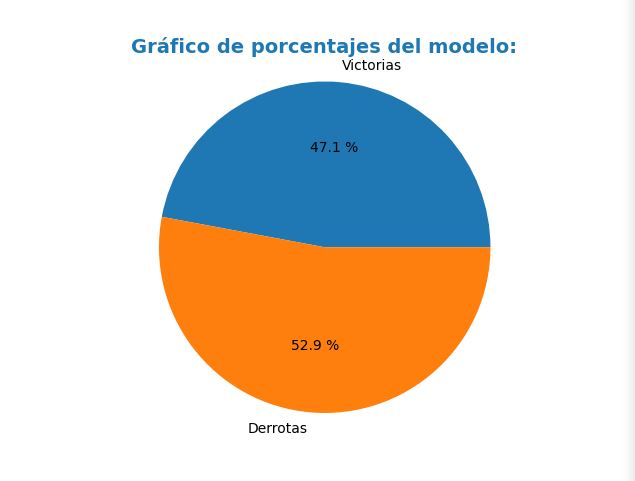
\includegraphics[width=0.3\textwidth]{mg1.JPG}
    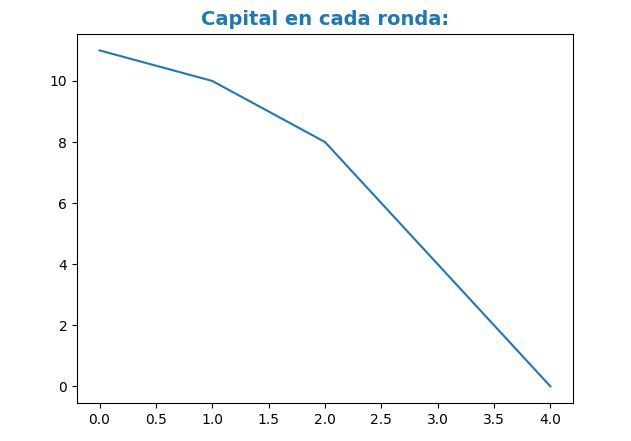
\includegraphics[width=0.3\textwidth]{mg2.JPG}

    \vspace{1cm}

    {\itshape\Large Estrategia D’Alembert \par}

    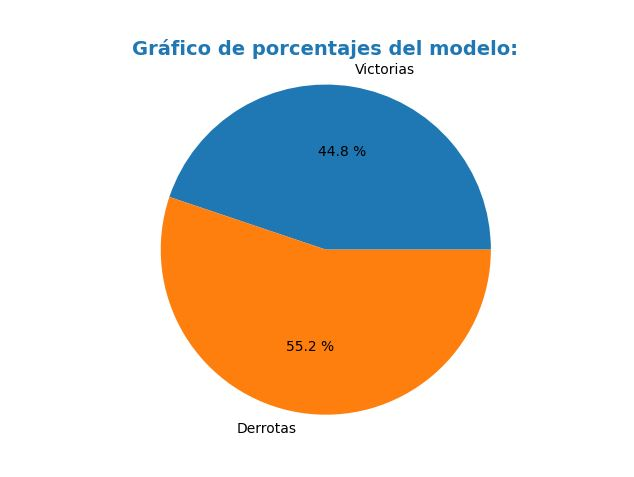
\includegraphics[width=0.3\textwidth]{dalem1.JPG}
    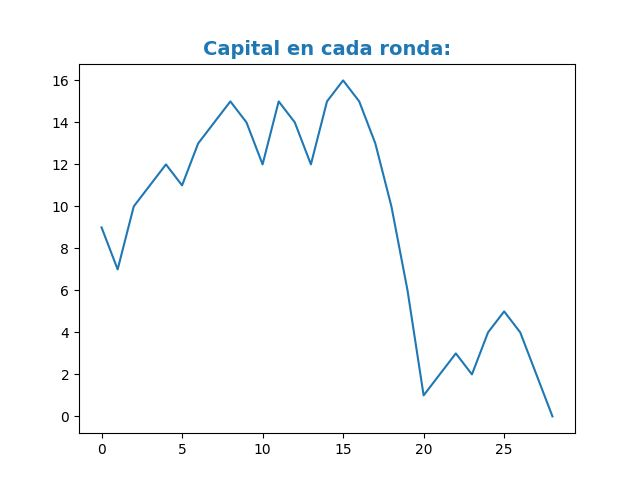
\includegraphics[width=0.3\textwidth]{dalem2.JPG}

    \vspace{1cm}

    {\itshape\Large Estrategia Fibonacci \par}

    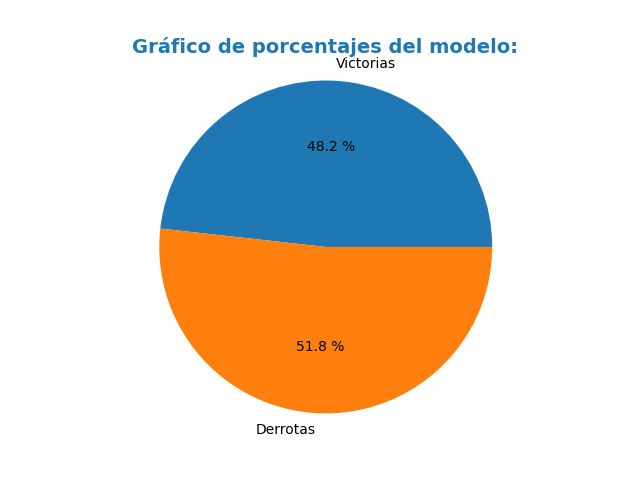
\includegraphics[width=0.3\textwidth]{fibo1.JPG}
    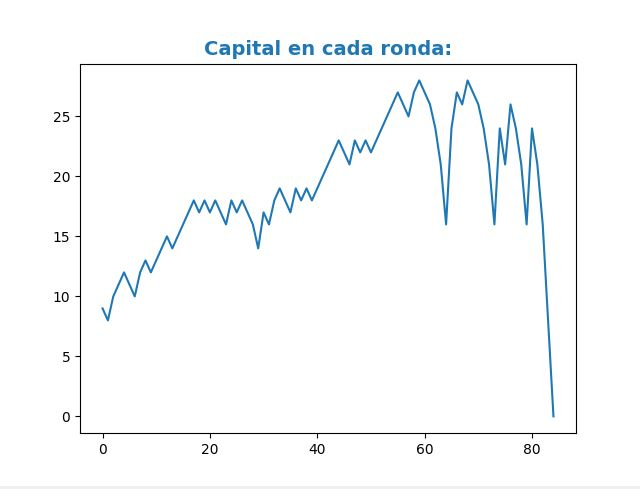
\includegraphics[width=0.3\textwidth]{fibo2.JPG}

    \vspace{1cm}

    {\itshape\Large Resumen de tiradas \par}
    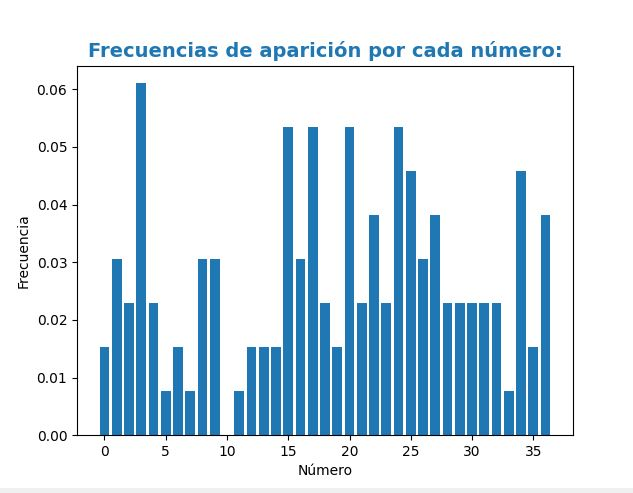
\includegraphics[width=0.3\textwidth]{frecAparicion.JPG}
    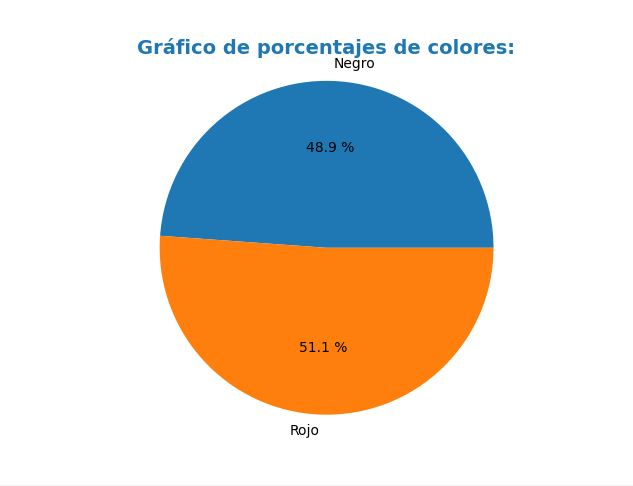
\includegraphics[width=0.3\textwidth]{resumenColores.JPG}

    \section{Conclusiones}

    Con lo obtenido y trabajado hasta el momento,
    el sistema más ganador en las tiradas correspondientes, es el denominado "Martingala",
    el cual posee el mayor porcentaje de victorias (52.9).
    La diferencia también se puede observar en los graficos de capital de cada ronda de los tres sistemas, donde
    en los otros sistemas, la curva decrece a comparación del primero. Se puede observar además, que el color rojo tiene más tendencia a salir,
    y que además, el los números que han más han salido, son los números que van desde el 15 al 25.



\end{document}
